\documentclass[12pt]{book}

% Packages
\usepackage{graphicx}
\usepackage{a4wide}
\usepackage{fancyhdr}
\usepackage{fancyvrb}
\usepackage{amsmath}
\usepackage{amssymb}
\usepackage{amsthm}
\usepackage{psfrag}
\usepackage{makeidx}
\usepackage{longtable}
\usepackage{here}
\usepackage{array}
\usepackage{algorithm}
\usepackage{algorithmicx}
\usepackage{algpseudocode}
\usepackage[procnames]{listings}
\usepackage[usenames]{color}
\usepackage{moreverb}
\usepackage{fancyvrb}
\usepackage{bm}
\usepackage{algorithm}
\usepackage{multicol}
\usepackage{url}
\usepackage{subfigure}
\usepackage{changepage}

% Set margins
\usepackage[top=3cm, bottom=3cm, left=3cm, right=3cm]{geometry} 

% Fonts and chapter styles
\usepackage{sectsty}
\sectionfont{\sf}
\subsectionfont{\it}
\usepackage[Sonny]{fncychap}
\usepackage{newcent}
\lhead{}
\rhead{}

% Clear empty page when chapter open right
\let\origdoublepage\cleardoublepage
\newcommand{\clearemptydoublepage}{%
  \clearpage
  {\pagestyle{empty}\origdoublepage}%
}

% Book macros
\newcommand{\fenicschapter}[4]{\chapter{#1 \\ \small{\rm By #3}} \vspace{-1cm}
                              Chapter ref: \textbf{[#4]} \label{chap:#4} \vspace{1cm} \chead[#2]{#3}}
\newcommand{\fenicsappendix}[2]{\chapter{#1} \chead{#2}}
\newcommand{\fenics}{\textbf{FEniCS}}
\newcommand{\dolfin}{\textbf{DOLFIN}}
\newcommand{\editornote}[1]{\noindent\begin{minipage}{\textwidth}
                            \small\it $\blacktriangleright$ \underline{\emph{Editor note}}: #1
                            \end{minipage}\normalsize \vspace{0.2cm}}
\newcommand{\authornote}[1]{\noindent\begin{minipage}{\textwidth}
                            \small\it $\blacktriangleright$ \underline{\emph{Author note}}: #1
                            \end{minipage}\normalsize \vspace{0.2cm}}
\newcommand{\includechapter}[1]}}

\fenicschapter{Improved Boussinesq Equations for Surface Water Waves}
              {Improved Boussinesq Equations for Surface Water Waves}
              {Nuno D. Lopes, P. J. S. Pereira and L. Trabucho}
              {lopes}

\editornote{Move macros to common macros after deciding what
              to do about bold fonts.}
\authornote{We have replaced  bold fonts  with
vector notation (e.g.: \({\bf u}\) changed to \(\vec{u}\)).}
\editornote{List authors with full names}

%{{{Abstract

The main motivation of this work is the implementation of a general
solver for some of the improved Boussinesq models\index{Boussinesq
models}.  Here, we use the second order model proposed by Zhao et al.
\cite{ZhaoTengEtAl2004} to investigate the behaviour of surface water waves.
Some effects like surface tension, dissipation and wave generation by
natural phenomena or external physical mechanisms are also included.
As a consequence, some modified dispersion relations are derived for
this extended model.
%}}}

%{{{ Introduction

\section{Introduction}

The \fenics\, project, via \dolfin\, and \ffc, provides a good
support for the implementation of large scale industrial models.  We
implement a solver for some of the Boussinesq type systems to model
the evolution of surface water waves\index{water waves} in a variable
depth seabed.  This type of models is used, for instance, in harbour
simulation\footnote{See Fig. \ref{lopes:fig:harbour} for an example of a
standard harbour.}, tsunami generation and propagation as well as in
coastal dynamics.
\begin{figure}[!htb]
\centering
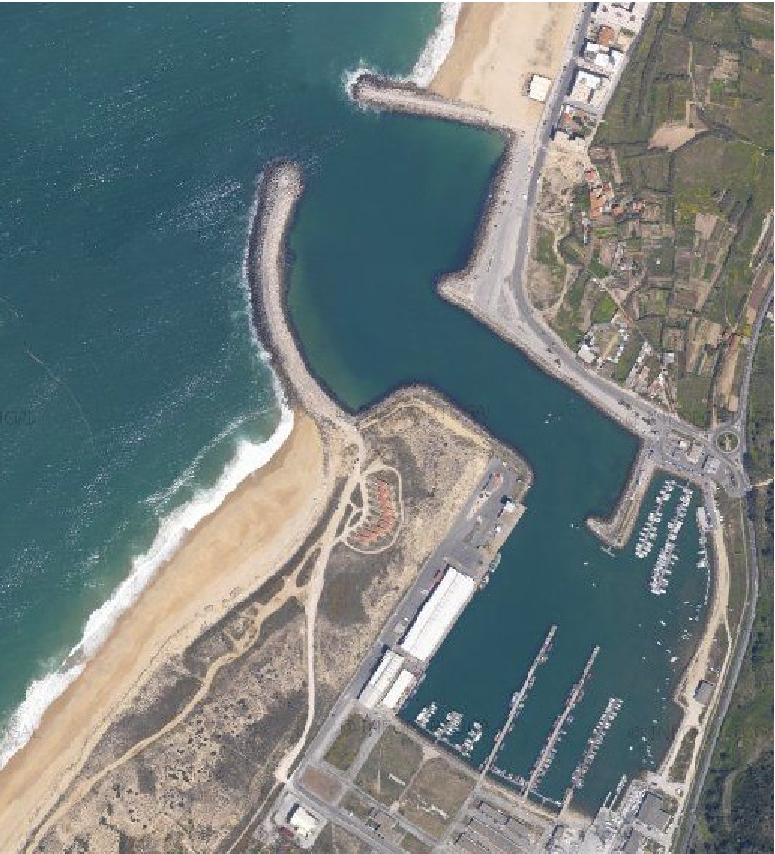
\includegraphics[width=\smallfig]{chapters/lopes/pdf/nazare1.pdf}
\caption{Nazar\'{e}'s harbour, Portugal.}\label{lopes:fig:harbour}
\end{figure}

\editornote{Need to get permission for this figure!}

There are several {\bf B}oussinesq models and some of the most widely
used are those based on the wave {\bf E}levation and horizontal {\bf
V}elocities formulation (BEV) (see, e.g., \cite{LiuWoo2004},
\cite{WalkleyBerzins2002}).

In the next section the governing equations for surface water waves
are presented. From these equations different types of models can be
derived.  We consider only the wave {\bf E}levation and velocity {\bf
P}otential (BEP) formulation.  Thus, the number of system equations is
reduced when compared to the BEV models.  Two different types of BEP
models are taken into account:
\begin{itemize}
\item[{\it i})] a standard sixth-order model (see subsection \ref{lopes:subsec:6th});
\item[{\it ii})] the second-order model proposed by {\bf Z}hao, {\bf T}eng
and {\bf C}heng (ZTC)  \cite{ZhaoTengEtAl2004} (see subsection \ref{lopes:subsec:ztc}).
\end{itemize}
We use the sixth-order model to  illustrate a standard
technique in order to  derive a  Boussinesq-type model.
In the subsequent sections, only the ZTC model is
considered.
Note  that these two models
 are complemented with some extra terms, due to the
inclusion of effects like dissipation, surface tension and  wave
generation by moving an impermeable bottom or using a source function.

An important characteristic of the modified ZTC model,
including dissipative effects,
is presented in the third section, namely,
 the dispersion relation.

In the fourth and fifth sections, we describe several types of
wave generation, absorption and reflection mechanisms.
Initial conditions for a solitary wave  and a periodic wave
induced by Dirichlet boundary conditions are also presented.
Moreover, we  complement the ZTC model using a  source
function  to generate surface water waves, as  proposed in \cite{WeiKirbyEtAl1999}.
Total reflective walls are modelled by standard zero Neumann
conditions for the surface elevation and velocity potential.
The wave energy absorption is simulated using sponge layers.

The following section is dedicated to the
numerical methods used in the discretization of the
variational formulation.
The discretization of the spatial variables  is accomplished
with low order Lagrange finite elements  whereas   the time integration
is implemented using  Runge-Kutta and Predictor-Corrector algorithms.

In the seventh section,  the ZTC numerical
model is used to simulate
the evolution of a periodic wave in an harbour  geometry  like that one represented in Fig. \ref{lopes:fig:harbour}.
%}}}

%{{{ Model derivation

\section{Model derivation}
As usual  we consider the following set of
equations for the irrotational flow of an incompressible and inviscid fluid:
\begin{equation}\label{lopes:eq:euler}
\begin{cases}
\displaystyle\fpar{ \vec{u}}{
  t}+(\vec{u}\cdot\nabla_{xyz})\vec{u}=-\nabla_{xyz}\left(\frac{P}{\rho} +g\, z\right),\\
\nabla_{xyz}\times \vec{u}={\vec{0}},  \\
\nabla_{xyz}\cdot{\vec{u}}=0,
\end{cases}
\end{equation}
where \(\vec{u}\) is the  velocity vector field of the fluid, \(P\) the
pressure, \(g\) the gravitational acceleration, \(\rho\) the
mass per unit volume, \(t\) the time and the differential operator \(\displaystyle\nabla_{xyz}=~\left[\fpar{}{x},\fpar{}{y},\fpar{}{z}\right]\!\!.\)
A Cartesian coordinate system is adopted with the
horizontal  \(x\) and \(y\)-axes on the still water plane and
the \(z\)-axis pointing vertically upwards
(see Fig. \ref{lopes:fig:schematic}). The fluid domain is
bounded by the  bottom seabed at \(z=-h(x,y,t)\) and the free
water surface at \(z=\eta(x,y,t)\).
%\editornote{AL: Need to decide what to do about bold fonts for vectors. I prefer not to use it.}
\begin{figure}[!htb]
{\centering
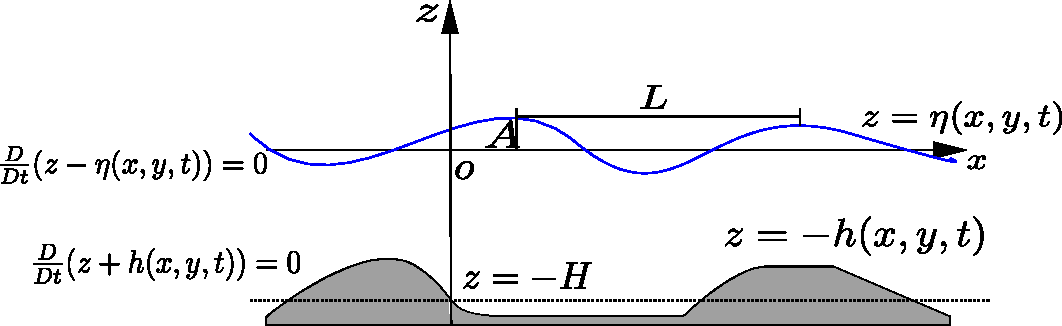
\includegraphics[width=\largefig]{chapters/lopes/pdf/graph.pdf}
\caption{Cross-section of the water wave domain.}\label{lopes:fig:schematic}
\par}
\end{figure}
In Fig. \ref{lopes:fig:schematic}, \(L\), \(A\) and \(H\) are
the characteristic wave length, wave amplitude and
depth, respectively. Note that the material time derivative is
denoted by \(\frac{D}{D t}\).

From the irrotational assumption (see \eqref{lopes:eq:euler}\(_2\)), one can  introduce a
velocity potential function, \(\phi(x,y,z,t)\)\index{potential}, to obtain  Bernoulli's equation:
\begin{equation}\label{lopes:eq:bern}
\fpar{ \phi}{ t}+\frac{1}{2}\nabla_{xyz} \phi \cdot\nabla_{xyz} \phi
+\frac{P}{\rho} +g\, z=f(t),
\end{equation}
where \(f(t)\) stands
for  an arbitrary function of integration.
 Note that one can   remove
 \(f(t)\)  from equation \eqref{lopes:eq:bern} if  \(\phi\) is
 redefined by \(\phi+\int f(t)\, {\rm d}t\).
From the incompressibility condition
(see \eqref{lopes:eq:euler}\(_3\))
 the velocity potential  satisfies  Laplace's equation:
\begin{equation}\label{lopes:eq:laplace}
\nabla^2\phi+\fpar{^2\phi}{z^2}=0,
\end{equation}
where \(\nabla\) is the  horizontal gradient operator given
by \(\displaystyle \nabla=\left[\fpar{}{x},\fpar{}{y}\right]\!\!.\)
To close this problem,  the following boundary conditions
must be satisfied:
\begin{enumerate}
\item[{\it i})]  the kinematic boundary condition for the free water surface:
\begin{equation}
\fpar{\phi}{z}=\fpar{\eta}{t}+\nabla\phi\cdot\nabla\eta,\quad z=\eta;
\end{equation}
\item[{\it ii})] the kinematic boundary condition for the impermeable sea bottom:
\begin{equation}
\fpar{\phi}{z}+(\nabla\phi\cdot\nabla h)=-\fpar{h}{t},
\quad z=-h ;
\end{equation}
\item[{\it iii})] the dynamic boundary condition for the free
water surface:
\begin{equation}\label{lopes:eq:dyn}
\fpar{\phi}{t}+ g\eta+\frac{1}{2}
\left(|\nabla\phi|^2 +\left(\fpar{\phi}{z}\right)^2\right)+
D(\phi)-W(\eta) = 0,
\quad z =\eta,
\end{equation}
\end{enumerate}
where \(D(\phi)\) is a  dissipative term (see, e.g., the work by Duthyk and
Dias \cite{DutykhDias2007}).
We assume that this dissipative term
 is of the following form:
\begin{equation}\label{lopes:eq:diss}
 D(\phi)=\nu\fpar{^2\phi}{z^2},
\end{equation}
with  \(\nu=\bar{\mu}/\rho\)  and \(\bar{\mu}\) an
 eddy-viscosity coefficient.
 Note that a
non-dissipative model means that there is no energy loss.
This is not acceptable from a physical point of view, since
any real flow is accompanied by energy dissipation.

In equation \eqref{lopes:eq:dyn}, \(W(\eta)\)  is the surface tension term given by:
\begin{equation}\label{lopes:eq:tension}
 \displaystyle W(\eta)=T\frac{\displaystyle \left(1+\left(\fpar{\eta}{y}\right)^2\right)\fpar{^2\eta}{x^2}+\left(1+\left(\fpar{\eta}{x}\right)^2\right)\fpar{^2\eta}{y^2}
-2\fpar{\eta}{x}\fpar{\eta}{y}\fpar{^2\eta}{\displaystyle x\partial
y}}{(1+|\nabla\eta|^2)^{3/2}},
\end{equation}
where \(T\) is the surface tension coefficient.

Using  Laplace's equation (see \eqref{lopes:eq:laplace}) it
is possible to rewrite \eqref{lopes:eq:diss}
as \(D(\phi)=-\nu\nabla^2\phi\).
Throughout the literature,  analogous terms were
added to the kinematic and dynamic conditions to
absorb the wave energy near  the boundaries.
These terms  are related with  the sponge or damping layers and, as we will
see later, they can be used to modify the dispersion relations.
In addition,  the linearization of equation \eqref{lopes:eq:tension}
results in \(W(\eta)=T\nabla^2\eta\).
The surface tension effects are important if short waves are considered.
Although the long wave assumption is made to derive
these extended models, waves of short length are generated in
the  domain due to the waves interaction.
Thus, the inclusion of surface tension  in the
small amplitude long wave models may be relevant.
On the other hand,  it is  worth to mention
that one of the main goals of the scientific research on Boussinesq
wave models is the  improvement  of the range of
applicability in terms of
the water-depth/wave-length relationship.
 We refer the works by Wang et
al. \cite{WangWuEtAl2008} as well as  Dash and Daripa  \cite{DashDaripa2002},
which included surface tension effects in the  KdV
(Korteweg-de Vries) and Boussinesq equations.

A more detailed description of the above equations is found
in  G. B. Whitham's reference book on waves \cite{Whitham1974},
or in the more recent book  by R. S. Johnson \cite{Johnson1997}.

%}}}

%{{{ Standard models

\subsection{Standard models}\label{lopes:subsec:6th}
In this subsection, we present  a generic  Boussinesq
system  using the velocity potential formulation.
To transform
equations \eqref{lopes:eq:bern}-\eqref{lopes:eq:tension} in a
dimensionless form, the following scales are
introduced:
\begin{equation}
( x', y')=\frac{1}{L}(x,y),\quad
z'=\frac{z}{H}, \quad  t'=\frac{t\sqrt{gH}}{L},\quad
 \eta'=\frac{\eta}{A},\quad  \phi'=
\frac{H\phi}{AL\sqrt{gH}},\quad h'=\frac{h}{H},
\end{equation}
together with the  small parameters
\begin{equation}
\mu=\frac{H}{L},\quad \varepsilon=\frac{A}{H}.
\end{equation}
In the last equation, \(\mu\) is usually called the
long wave parameter  and \(\varepsilon\) the
small amplitude wave parameter.
Note that \(\varepsilon\)
is  related with the nonlinear terms and \(\mu\) with the
dispersive terms.
For simplicity, in what follows, we drop the prime notation.

The Boussinesq approach consists in reducing a 3{\bf D}
problem to a 2{\bf D} one.
This may be accomplished by
 expanding the
velocity potential in a Taylor power series in terms of \(z\).
Using  Laplace's
equation, in a dimensionless form, one can obtain the
following  expression for the velocity potential:
\begin{equation}
\phi(x,y,z,t)=\sum_{n=0}^{+\infty}\left((-1)^n\frac{z^{2n}}{(2n)!}\mu^{2n}\nabla^{2n}\phi_0(x,y,t)+
(-1)^n \frac{z^{2n+1}}{(2n+1)!}\mu^{2n}\nabla^{2n}\phi_1(x,y,t)\right),
\end{equation}
with
\begin{equation}
\phi_0=\phi\mid_{ z=0},\quad \phi_1=\left(\fpar{\phi}{z}\right)\mid_{z=0}\!.
\end{equation}
From asymptotic expansions,  successive approximation
techniques and the kinematic boundary condition for the sea bottom, it is possible to
write \(\phi_1\)   in terms of \(\phi_0\) (cf. \cite{ChenLiu1994}, \cite{ZhaoTengEtAl2004}).
In this work, without loss of generality,  we  assume that
the dispersive and nonlinear terms are related by the
following equation:
\begin{equation}
\frac{\varepsilon}{\mu^2}=O(1).
\end{equation}
Note that  the Ursell number is defined by \(\displaystyle
U_r=\frac{\varepsilon}{\mu^2}\).

A sixth-order model is obtained if
 \(\phi_1\) is expanded in terms of \(\phi_0\) and all terms
up to \(O(\mu^8)\) are retained.
Thus,  the asymptotic kinematic and dynamic
boundary conditions for the free water surface  are
rewritten as
 follows \footnote{Note that \(D\)
and \(W\) are, now,   dimensionless functions.}:
\begin{equation}\label{lopes:eq:kindyn}
\renewcommand{\arraystretch}{1.7}
\left\{\begin{array}{l}
\displaystyle\fpar{\eta}{t}+\varepsilon\nabla\cdot(\eta\nabla\phi_0)-\frac{1}{\mu^2}\phi_1+
\frac{\varepsilon^2}{2}\nabla\cdot(\eta^2\nabla\phi_1)=O(\mu^{6}),
\vspace{0.3cm}
\\
\displaystyle \fpar{\phi_0}{t}+\varepsilon\eta\fpar{\phi_1}{t}+\eta +
\frac{\varepsilon}{2} \left|\nabla\phi_0\right|^2+\varepsilon^2\nabla\phi_0\cdot\eta\nabla\phi_1-\\
\displaystyle \qquad -\varepsilon^2\eta\nabla^2\phi_0\phi_1
+\frac{\varepsilon}{2\mu^2}\phi_1^2
+D(\phi_0,\phi_1)-W(\eta)
=O(\mu^{6}),
\end{array}\right .
\end{equation}
where \(\phi_1\) is given by:
\begin{multline}\label{lopes:eq:phi_1}
\phi_1=
-\mu^{2}\nabla\cdot\left(h\nabla\phi_0\right)
+\frac{\mu^{4}}{6}\nabla\cdot\left(h^3\nabla^3\phi_0\right)
-\frac{\mu^{4}}{2}\nabla\cdot\left(h^2
\nabla^2\cdot\left(h\nabla\phi_0\right) \right)-\\
-\frac{\mu^6}{120}\nabla\cdot\left(h^5\nabla^5\phi_0\right)+
\frac{\mu^6}{24}\nabla\cdot\left(h^4\nabla^4\cdot\left(h\nabla\phi_0\right)\right)+\frac{\mu^6}{12}\nabla\cdot\left(h^2\nabla^2\cdot\left(h^3\nabla^3\phi_0\right)\right)-\\
-\frac{\mu^6}{4}\nabla\cdot\left(h^2\nabla^2\cdot\left(h^2\nabla^2\cdot\left(h\nabla\phi_0\right)\right)\right)
-\frac{\mu^2}{\varepsilon}\fpar{h}{t}-
\frac{\mu^2}{\varepsilon}\frac{\mu^2}{2}\nabla\cdot\left(h^2\nabla\fpar{h}{t}\right)+\\
+\frac{\mu^2}{\varepsilon}\frac{\mu^4}{24}\nabla\cdot\left(h^4\nabla^3
\fpar{h}{t}\right)
-\frac{\mu^2}{\varepsilon}\frac{\mu^4}{4}\nabla\cdot\left(h^2\nabla^2\left(h^2\nabla\fpar{h}{t}\right)\right)+O(\mu^{8}).
\end{multline}
To obtain equation \eqref{lopes:eq:phi_1}, we assume
that \(\displaystyle\fpar{h}{t}=O(\varepsilon)\) (cf. \cite{DutykhDias2007}).

%}}}

%{{{ \(2^{nd}\)-order model

\subsection{Second-order model}\label{lopes:subsec:ztc}
The low order equations are obtained, essentially, via
the slowly varying bottom assumption. In
particular, only  \(O(h,\nabla h)\) terms are
retained.
Also, only low order  nonlinear terms, \(O(\varepsilon)\), are admitted.
In fact, the modified ZTC model is  written retaining
only \(O(\varepsilon,\mu^4)\) terms.

Under these conditions,  \eqref{lopes:eq:kindyn}
and \eqref{lopes:eq:phi_1} lead to:
\begin{equation}\label{lopes:eq:kindyn2}
\begin{cases}
\displaystyle\fpar{\eta}{t}+\varepsilon\nabla\cdot(\eta\nabla\phi_0)-\frac{1}{\mu^2}\phi_1=O(\mu^{6}),\vspace{0.3cm} \\
\displaystyle\fpar{\phi_0}{t}+\eta +
\frac{\varepsilon}{2} \left|\nabla\phi_0\right|^2-\nu^*\varepsilon\nabla^2\phi_0-T^*\mu^2\nabla^2\eta
=O(\mu^{6}),
\end{cases}
\end{equation}
where \(\nu^*=\nu\sqrt{H}/(AL\sqrt{g})\), \(T^*= T/(gH^2)\)
and
\begin{multline}\label{lopes:eq:phi_2}
\phi_1=
-\mu^{2}\nabla\cdot\left(h\nabla\phi_0\right)
+\frac{\mu^{4}}{6}\nabla\cdot\left(h^3\nabla^3\phi_0\right)
-\frac{\mu^{4}}{2}\nabla\cdot\left(h^2
\nabla^2\cdot\left(h\nabla\phi_0\right) \right)-\\
-\frac{2\mu^6}{15}h^5\nabla^6\phi_0-2\mu^6h^4\nabla h\cdot\nabla^5\phi_0
-\frac{\mu^2}{\varepsilon}\fpar{h}{t}+O(\mu^{8}).
\end{multline}
Thus, these extended equations, in terms of the dimensional
variables, are written as follows:
\begin{equation}\label{lopes:eq:ztc}
\begin{cases}
\displaystyle \frac{\partial\eta}{\partial t} +\nabla\cdot[(h+\eta)\nabla{\Phi}]
-\frac{1}{2}\nabla\cdot [h^{2}\nabla\frac{\partial \eta}
{\partial t}]
+\frac{1}{6}h^{2}\nabla^2\frac{\partial\eta}{\partial t}
-\frac{1}{15}\nabla\cdot[h\nabla(h\frac{\partial\eta}
{\partial t})]=-\fpar{h}{t},\vspace{0.3cm} \\
\displaystyle \frac{\partial \Phi}{\partial t}
+\frac{1}{2}|\nabla\Phi|^2+g\eta-
\frac{1}{15}gh\nabla\cdot(h\nabla\eta)-\nu\nabla^2\Phi-T\nabla^2\eta=0,
\end{cases}
\end{equation}
where  \(\Phi\) is  the transformed velocity potential given
by:
\begin{equation}\label{lopes:eq:phitrans}
\Phi=\phi_0+\frac{h}{15}\nabla\cdot(h\nabla\phi_0) .
\end{equation}
 The transformed velocity potential
is used with two main consequences  (cf. \cite{ZhaoTengEtAl2004}):
\begin{itemize}
\item[{\it i})]  the  spatial derivation order is reduced to the
second order;
\item[{\it ii})] linear dispersion characteristics,
analogous to the fourth-order BEP model proposed by Liu and Woo
 \cite{LiuWoo2004} and  the third-order BEV model  developed
by  Nwogu  \cite{Nwogu1993}, are obtained.
\end{itemize}

%}}}

%{{{ Linear dispersion relation

\section{Linear dispersion relation}
One of the most important properties of a water  wave model is
described by the linear dispersion relation.
From this relation we can deduce the phase velocity, group velocity
and the linear shoaling.
The dispersion relation\index{dispersion relation} provides
a good method to characterize the linear
properties of a wave model.
This is achieved using the linear wave
theory of Airy.

In this section we follow the  work by Duthyk and
Dias \cite{DutykhDias2007}.
Moreover, we  present a generalized version of the dispersion
relation for the ZTC model with the
dissipative term mentioned above.
One can also include other damping terms, which are usually
used in the sponge layers.

For simplicity,  a 1{\bf D}-Horizontal  model is  considered.
To obtain the dispersion relation,
a standard  test  wave is assumed:
\begin{equation}\label{lopes:eq:linwave}
\begin{cases}
\eta(x,t)=a\,e^{i(kx-\omega t)},\vspace{0.3cm}\\
\Phi(x,t)=-b\,i\,e^{i(kx-\omega t)},
\end{cases}
\end{equation}
where \(a\) is the wave amplitude,  \(b\) the potential
magnitude, \(k=2\pi/L\) the wave number and \(\omega\) the angular frequency.
This wave, described by equations \eqref{lopes:eq:linwave}, is the
solution of the linearized  ZTC model, with a constant depth
bottom and an extra dissipative term,
 if the following equation is satisfied:
\begin{equation}\label{lopes:eq:dissdisp}
\omega^2-ghk^2\frac{1+(1/15)(kh)^2}{1+2/5(kh)^2}+i\nu\omega k^2=0.
\end{equation}
Using Pad\'{e}'s [2,2] approximant,  the dispersion relation
given by last equation  is accurate up to \(O((kh)^4)\) or \(O(\mu^4)\) when
compared with the following equation:
\begin{equation}\label{lopes:eq:linairy}
\omega^2-ghk^2\frac{\tanh(kh)}{kh}+i\nu\omega k^2=0.
\end{equation}
In  fact, equation \eqref{lopes:eq:linairy} is the dispersion
relation of the full linear problem.

From \eqref{lopes:eq:dissdisp}, the
 phase velocity, \(\displaystyle C=\frac{w}{k}\),  for this dissipative ZTC model is
 given by:
\begin{equation}
C=-\frac{i\nu k}{2}\pm\sqrt{-\left(\frac{\nu k}{2}\right)^2+gh\frac{(1+1/15(kh)^2)}{(1+2/5(kh)^2)}}.
\end{equation}
In Fig. \ref{lopes:fig:dispersion}, we can see the positive real
part
of \(\displaystyle\left(C/\sqrt{gh}\right)\) as a function of \(kh\) for the following models:
  full linear theory (FL),
Zhao et al. (ZTC), full linear theory with a
dissipative model (FL\_D) and the
improved  ZTC model with the dissipative term (ZTC\_D).
\begin{figure}[htb]
  \begin{center}
    %\psfrag{Re}[lb][lb]{$Re\left(C/\sqrt{gh}\right)$}
    %\psfrag{kh}[lt][lt]{$kh$}
    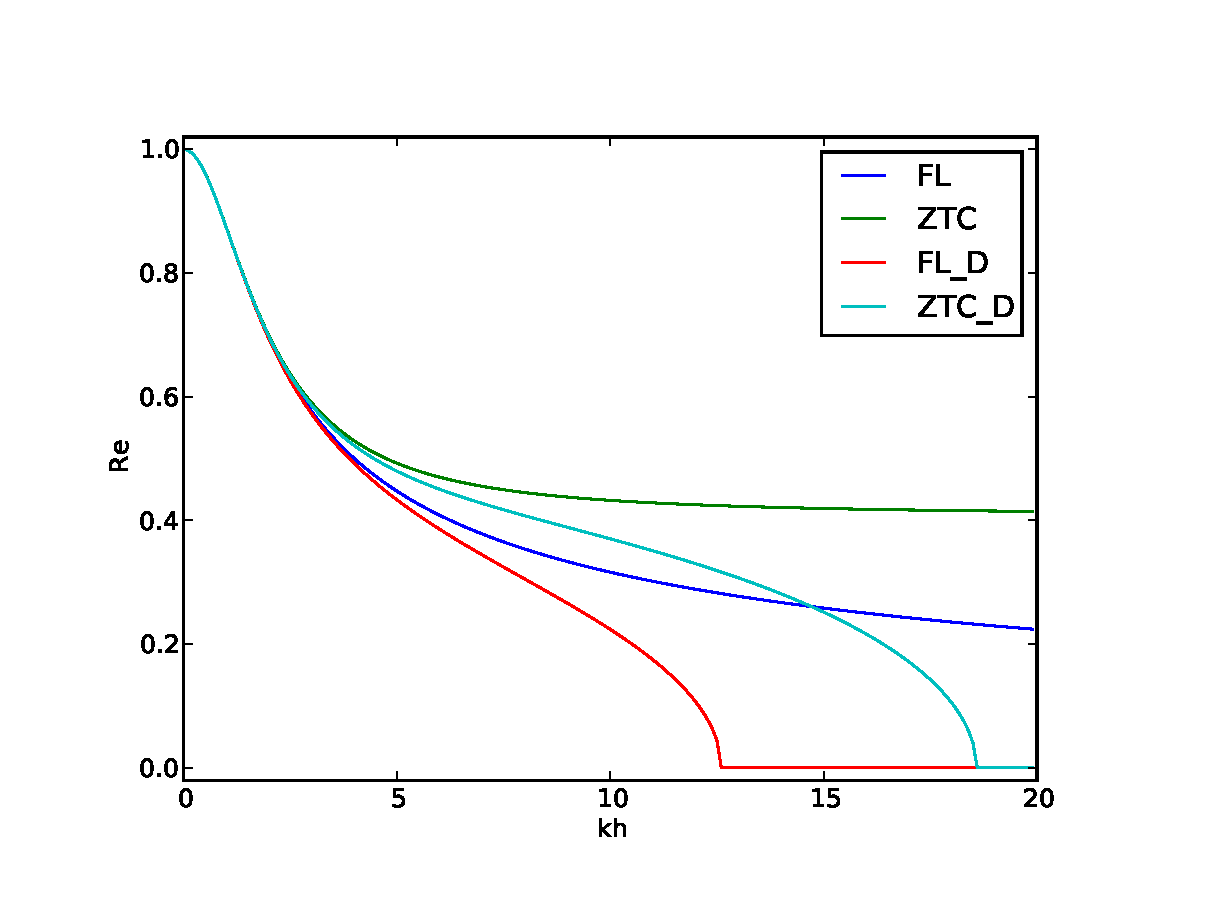
\includegraphics[width=\largefig]{chapters/lopes/pdf/dispersion.pdf}
    \caption{Positive  part of $Re C/ \sqrt{gh}$ as a function of $kh$ for several models.}
    \label{lopes:fig:dispersion}
  \end{center}
\end{figure}
From Fig. \ref{lopes:fig:dispersion}, one can also see that
  these two dissipative models  admit
critical wave numbers \(k_1\) and \(k_2\),
such that the positive  part of \(\displaystyle Re\left(C/\sqrt{gh}\right)\) is zero
for \(k\geq k_1\) and \(k\geq k_2\).
To avoid some numerical instabilities one can optimize
 the \(\nu\) values in order
 to reduce  the short waves propagation.


In general, to improve the dispersion relation one can also use other
 transformations like \eqref{lopes:eq:phitrans}, or evaluate the
 velocity potential at \(z=-\sigma h\) (\(\sigma\in[0,1]\))
 instead of  \(z=0\) (cf. \cite{BinghamMadsenEtAl2008}, \cite{MadsenAgnon2003} and \cite{MadsenBinghamEtAl2003}).

%}}}

%{{{ Wave generation
\section{Wave generation}
In this section some of the physical mechanisms to induce
surface water waves are presented.
We note that the moving bottom approach is useful for wave
generation due to seismic activities. However, some
physical applications  are associated with other wave generation mechanisms.
For simplicity, we only consider
mechanisms to generate surface water waves
along the \(x\) direction.

\subsection{Initial condition}
The simplest way of inducing a wave into a certain domain is
to consider an appropriate initial condition.
An useful and typical benchmark case
is to assume a solitary wave given by:
\begin{equation}
\eta(x,t)=a_1\,{\rm sech}^2(kx -\omega t)+a_2\,{\rm
sech}^4(kx-\omega t),
\end{equation}
\begin{equation}
u(x,t)=a_3\,{\rm sech}^2(k x-\omega t),
\end{equation}
where the parameters \(a_1\) and \(a_2\) are the wave amplitudes and \(a_3\) is the magnitude
of the velocity in the \(x\) direction.
As we   use a potential formulation, \(\Phi\) is given by:
\begin{equation}
\Phi(x,t)=-\frac{2a_3\,e^{2\omega t }}{k\,(e^{2\omega t
}+e^{2k x})}+ K_1(t),
\end{equation}
where   \(K_1(t)\) is
a time-dependent  function of integration.

In \cite{Walkley1999} and \cite{WeiKirby1995} the above solitary wave was presented as a
solution of the extended Nwogu's Boussinesq
model.

\subsection{Incident wave}\label{lopes:subsec:incidentwave}
For time-dependent wave generation,
it is possible to consider waves induced by a boundary
condition.
This requires that the wave surface elevation and
the velocity potential must satisfy appropriated boundary
conditions, e.g.,
Dirichlet or Neumann conditions.\index{boundary conditions}

The simplest case is to consider  a periodic wave given by:
\begin{equation}\label{lopes:eq:eta}
\eta(x,t)=a \sin(kx-\omega t)
\end{equation}
\begin{equation}\label{lopes:eq:phi}
\Phi(x,t)=-\frac{c}{k}\cos(k x-\omega t)+K_2(t),
\end{equation}
where \(c\) is the wave velocity magnitude and \(K_2(t)\) is a time-dependent function of integration.
This function \(K_2(t)\) must satisfy   the initial
condition of the problem.
 In equations \eqref{lopes:eq:eta} as well as \eqref{lopes:eq:phi},
 one can note that  the parameters \(a,c,k\) and \(\omega\)  are
not all arbitrary, since they are related by the dispersion relation.
One can also consider the  superposition of water waves
as solutions of the full linear problem with a constant depth.
%}}}

%{{{ Source function

\subsection{Source function}
In  the work by Wei et
al.  \cite{WeiKirbyEtAl1999}, a source function\index{source function}
  for the  generation of surface water waves was derived.
This source function was obtained, using   Fourier
transform and Green's functions, to solve the  linearized and
non homogeneous equations of the
 Peregrine \cite{Peregrine1967} and  Nwogu's \cite{Nwogu1993} models.
This mathematical procedure can also be  adapted here  to
deduce the source function.

We  consider  a monochromatic
Gaussian wave generated by the following  function:
\begin{equation}\label{lopes:eq:src}
S(x,t)=D^* \exp(-\beta (x-x_s)^2)\cos(\omega t),
\end{equation}
with \(D^*\) given by:
\begin{equation}
\displaystyle D^*=\frac{\sqrt{\beta}}{\omega\sqrt{\pi}}a\exp(\frac{k^2}{4\beta})\frac{2}{15}h^3k^3g.
\end{equation}
In the above expressions
\(x_s\) is the center line of the source function and
\(\beta\)  is a parameter associated with the width of the
generation band (cf. \cite{WeiKirbyEtAl1999}).
%}}}

%{{{ Reflective walls and sponge layers
\section{Reflective walls and sponge layers}

Besides the incident wave boundaries
 where the wave profiles
are given, one must close the system with appropriate
boundary conditions.
We consider two more types of
boundaries:
\begin{itemize}
\item[{\it i})] full reflective boundaries;\index{reflective boundaries}
\item[{\it  ii})] partial reflective or absorbing boundaries.
\end{itemize}
The first case is modelled by the following equations:
\begin{equation}\label{lopes:eq:fullrefl}
\frac{\partial \Phi}{\partial \vec{n}}=0,\qquad\frac{\partial \eta}{\partial \vec{n}}=0,
\end{equation}
where \(\vec{n}\) is the outward unit vector normal to the
computational domain \(\Omega\).
We  denote  \(\Gamma\) as  the boundary of \(\Omega\).

Note that  in  the finite element formulation, the full
reflective boundaries (equations \eqref{lopes:eq:fullrefl})  are integrated by
considering zero Neumann-type boundary conditions.

Coupling the  reflective case and an extra artificial
  layer, often called sponge \index{sponge-layers} or damping layer,
we can simulate partial reflective or full absorbing boundaries.
In this way, the  reflected energy
can be controlled. Moreover, one can prevent unwanted wave
  reflections and avoid complex wave interactions.
It is also possible to simulate effects like energy dissipation by wave breaking.

In fact, a sponge layer is a
subset \(\Omega_S\) of \(\Omega\) where
some extra viscosity term is added.
As mentioned above, the system of equations can incorporate
several extra damping terms, like that one provided by the
inclusion of  a dissipative model. Thus, the viscosity
coefficient \(\nu\) can be described  by a
 function of the following form:
\begin{equation}
\nu(x,y)=
\left\{
\begin{matrix}
0,& (x,y)\not\in\Omega_S ,\vspace{0.3cm}\\
\displaystyle
n_1\frac{\displaystyle\exp{\left(\frac{d_{\Omega_S}-d(x,y)}{d_{\Omega_S}}\right)^{n_2}}-1}{\exp(1)-1},&
(x,y) \in\Omega_S,
\end{matrix}
\right.
\end{equation}
where \(n_1\) and  \(n_2\) are, in general, experimental
 parameters, \(d_{\Omega_S}\) is  the sponge-layer diameter and
 \(d(x,y)\)
stands for a distance function between a point \((x,y)\) and
 the intersection of \(\Gamma\) with the boundary
 of \(\Omega_S\) (see, e.g., \cite{Walkley1999}).
%}}}

%{{{ Numerical Methods

\section{Numerical Methods}
We start this section by noting that a detailed description
of  the implemented numerical methods referred bellow
can be found in the work of N. Lopes \cite{N.Lopes2007}.

For simplicity, we only consider
the second-order system described by
equations \eqref{lopes:eq:ztc}  restricted to a stationary
bottom and without
dissipative, surface tension or extra source terms.

The model variational formulation is written as follows:
\begin{equation}\label{lopes:eq:varform}
\renewcommand{\arraystretch}{2.0}
\left\{
\begin{array}{l}
\displaystyle \int_\Omega\fpar{\eta}{t}\fba\, \dx\dy
+\frac{1}{2}\int_\Omega
h^2\nabla\left(\fpar{\eta}{t}\right)\cdot\nabla\fba\, \dx\dy-
\frac{1}{6}\int_\Omega \nabla\left( \fpar{\eta}{t}\right)\cdot\nabla(h^2\fba)\, \dx\dy+\\
\quad \quad\displaystyle +
\frac{1}{15}\int_\Omega h\nabla\left(h\fpar{\eta}{t}\right)\cdot \nabla\fba\, \dx\dy-
\frac{1}{15}\int_\Gamma
h\fpar{h}{\vec{n}}\,\fpar{\eta}{t}\,\fba\, d\Gamma=
\quad\\\displaystyle
\int_\Omega(h+\eta)\nabla\Phi\cdot\nabla\fba\, \dx\dy
-\int_\Gamma(h+\eta)\fpar{\Phi}{\vec{n}}\fba\, d\Gamma
+\frac{2}{5}\int_\Gamma
h^2\fpar{}{t}\left(\fpar{\eta}{\vec{n}}\right)\fba d\Gamma,
\vspace{0.3cm} \\
\displaystyle \int_\Omega \fpar{\Phi}{t}\,\fbb\, \dx\dy=
-\frac{1}{2}\int_\Omega|\nabla\Phi|^2\fbb\, \dx\dy
-g\int_\Omega \eta\,\fbb\, \dx\dy-
\\
\quad\quad\displaystyle-\frac{g}{15}\int_\Omega h\nabla\eta\cdot\nabla(h\fbb)\, \dx\dy +\frac{g}{15}\int_\Gamma h^2\fpar{\eta}{\vec{n}}\,\fbb\, d\Gamma,
\end{array}
\right .
\end{equation}
where  the unknown functions
\(\eta\) and \(\Phi\) are the surface elevation and the
transformed velocity potential, whereas  \(\fba\) and \(\fbb\)
are the test functions defined in  appropriate spaces.

The spatial  discretization of these equations
is implemented  using low order  Lagrange finite elements.
In addition, the numerical implementation
of \eqref{lopes:eq:varform} is accomplished using  \ffc.

We use
a predictor-corrector \index{Predictor-Corrector}  scheme with an initialization
provided by an explicit Runge-Kutta\index{Runge-Kutta} method for the
time integration.
Note that the discretization of
equations \eqref{lopes:eq:varform} can be written in the following form:
\begin{equation}
M\dot U={\vec{F}}(t,U),
\end{equation}
where \(\dot U\) and \(U\) refer
to \(\displaystyle \left(\fpar{\eta}{t},\fpar{\Phi}{t}\right)\)
and  \((\eta,\Phi)\), respectively.
The  coefficient matrix \(M\) is given by the left-hand
sides of \eqref{lopes:eq:varform}, whereas
the  known vector \(\vec{F}\) is  related
with the right-hand sides of the same equations.
In this way,  the fourth order  Adams-Bashforth-Moulton method
can be written as follows:
\begin{equation}\label{lopes:eq:pc}
\renewcommand{\arraystretch}{1.3}
\left\{
\begin{array}{l}
\displaystyle MU^{(0)}_{n+1}=MU_n+\frac{\Delta
t}{24}[55{\vec{F}}(t_n,U_n)-59{\vec{F}}(t_{n-1},U_{n-1})+\\
\hspace{2.5in}+37{\vec{F}}(t_{n-2},U_{n-2})-9{\vec{F}}(t_{n-3},U_{n-3})],
\vspace{0.3cm}\\
\displaystyle MU^{(1)}_{n+1}=MU_n+\frac{\Delta
t}{24}[9{\vec{F}}(t_{n+1},U^{(0)}_{n+1})+19{\vec{F}}(t_n,U_n)-\\
\hspace{2.5in}-5{\vec{F}}(t_{n-1},U_{n-1})+{\vec{F}}(t_{n-2},U_{n-2})],
\end{array}
\right.
\end{equation}
where \(\Delta t\) is the time step, \(t_n=n\Delta
  t\) \((n\in \mathbb{N})\) and \(U_n\) is \(U\)
  evaluated at \(t_n\).
  The predicted and
corrected values of \(U_n\) are denoted by \(U_n^{(0)}\) and \(U_n^{(1)}\),  respectively.
The corrector-step equation (\eqref{lopes:eq:pc}\(_{2}\)) can
be iterated as  function of a predefined error
between consecutive time steps. For more details see, e.g.,  \cite{HairerWanner1991a}
or \cite{Lambert1991}.

%}}}

%{{{ Numerical Applications

\section{Numerical Applications}
In this section,
we present some numerical results about the propagation
 of surface water waves in an harbour with a geometry
similar to that one of  Fig. \ref{lopes:fig:harbour}.

The colour scale used in Figs. \ref{lopes:fig:harbour_depth}--\ref{lopes:fig:potential1}  is presented in
Fig. \ref{lopes:fig:scale}.
A schematic description of the fluid domain, namely the bottom profile and the
sponge layer can be seen in Figs. \ref{lopes:fig:harbour_depth}
and \ref{lopes:fig:sponge}, respectively.
Note that a piecewise linear bathymetry  is considered.
A sponge layer is used to absorb the wave energy at the
outflow region
and to avoid strong  interaction between incident and
reflected waves  in the harbour entrance.
 A monochromatic periodic wave
is introduced at the indicated boundary (Dirichlet BC) in
Fig. \ref{lopes:fig:sponge}.
This is achieved by considering waves induced by
a periodic Dirichlet boundary condition, as
described in the subsection \ref{lopes:subsec:incidentwave},
with the following characteristics:
\begin{center}
\renewcommand{\arraystretch}{1.3}
\begin{tabular}{|c|c|c|}
\hline
\(a\)       &   wave  amplitude &     \(0.25 \,{\tt m}\)\\ \hline
\(\omega\)  &   wave angular frequency       &   \(0.64715 \,{\tt s}^{-1}\)\\ \hline
\(p\)       &   wave  period  &       \(4.06614 \,{\tt s}\)\\ \hline
\(k\)       &   wave number &   \(0.06185 \,{\tt m}^{-1}\)\\ \hline
\(L\)       &   wave length &       \(101.59474 \,{\tt m}\)\\ \hline
\(b\)       &   wave potential magnitude&   \(3.97151 \,{\tt m}^2{\tt s}^{-1}\)\\ \hline
\(c\)       &   wave velocity  magnitude&  \(0.24562 \,{\tt m\, s}^{-1}\) \\ \hline
\(\varepsilon\)&   small amplitude parameter & \(0.01823\)\\ \hline
\(\mu\)     &   long wave parameter &       \(0.13501\)\\ \hline
\end{tabular}
\end{center}
Full reflective walls are assumed as boundary conditions in
all domain boundary except in the harbour entrance.
In Fig. \ref{lopes:fig:elevation}
a snapshot of the surface elevation  is shown at the time
 \(t_s=137\,{\tt s}\).

 A zoom of the image, which  describes
the physical potential \(\phi_0(x,y)\) and velocity vector field in the still
water plane, is given in  the neighbourhood of  the
point \(P_3=(255,-75)\,{\tt m}\) at \(t_s\) (see
Fig. \ref{lopes:fig:potential1}).
The Figs. \ref{lopes:fig:etap} and \ref{lopes:fig:velp} represent
 the surface elevation and water speed as a function of the
 time, at the
points \(P_1=(-350, 150)\,{\tt m},\, P_2=(-125,60)\,{\tt
m}\) and \(P_3\).
\begin{figure}[!htb]
\begin{minipage}[t]{0.3\linewidth}
%\psfrag{Xd3d 8.3.2 (15 Dec 2007)}[rb][rb]{}
%\psfrag{-0.1772}[lt][lt]{\(\longleftarrow\tt Max\)}
%\psfrag{-0.2052}[lt][lt]{}
%\psfrag{-0.2332}[lt][lt]{}
%\psfrag{-0.2612}[lt][lt]{}
%\psfrag{-0.2892}[lt][lt]{}
%\psfrag{-0.3172}[lt][lt]{}
%\psfrag{-0.3452}[lt][lt]{}
%\psfrag{-0.3732}[lt][lt]{}
%\psfrag{-0.4012}[lt][lt]{}
%\psfrag{-0.4292}[lt][lt]{}
%\psfrag{-0.4572}[lb][lb]{\(\longleftarrow\tt min\)}
{\centering
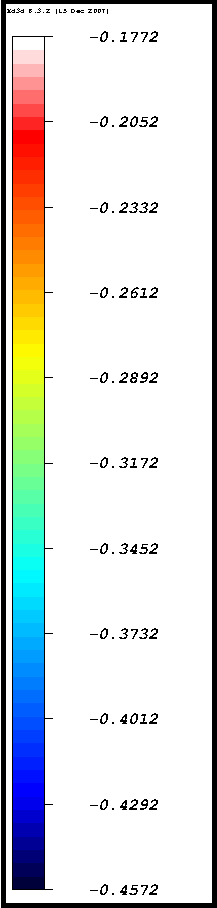
\includegraphics[width=1.5cm]{chapters/lopes/pdf/table.pdf}
\caption{Scale.}\label{lopes:fig:scale}\par}
\end{minipage}\hfill
\begin{minipage}[t]{0.7\linewidth}
{\centering
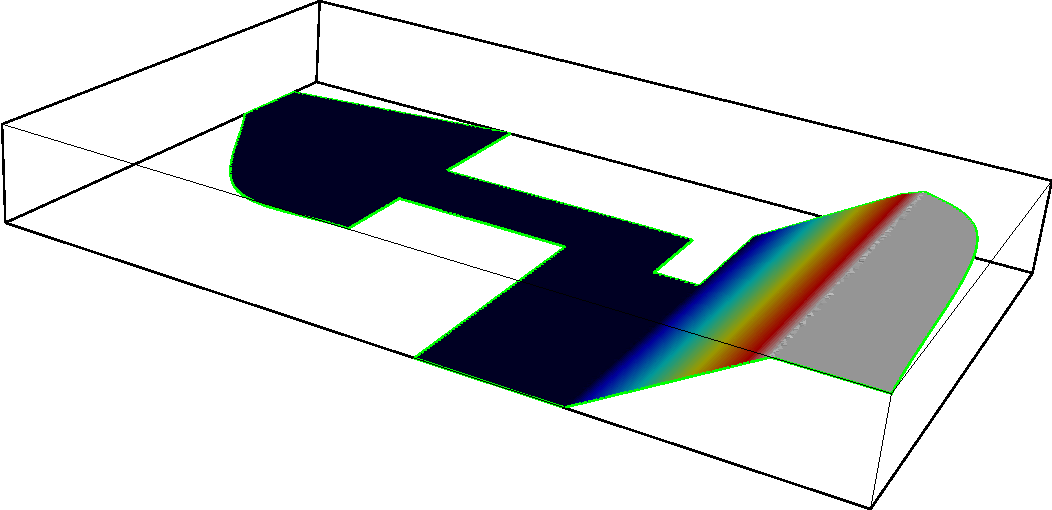
\includegraphics[width=\largefig]{chapters/lopes/pdf/depth.pdf}
\caption{Impermeable bottom $[{\tt Max}=-5.316\,{\tt m},{\tt min}=-13.716\,{\tt m}]$.}
\label{lopes:fig:harbour_depth}\par}
\end{minipage}
\end{figure}
\begin{figure}[htb!]
{\centering
%\psfrag{300}[rt][rt]{$y\, ({\tt m})$\,\,$300$}
%\psfrag{501}[rb][rb]{}
%\psfrag{200}[rb][rb]{}
%\psfrag{100}[rb][rb]{}
%\psfrag{301}[rb][rb]{}
%\psfrag{-100}[rb][rb]{}
%\psfrag{-200}[rb][rb]{}
%\psfrag{-300}[rb][rb]{}
%\psfrag{0}[rb][rb]{0}
%\psfrag{450}[rt][rt]{$-450$}
%\psfrag{360}[rt][rt]{$-360$}
%\psfrag{01}[rb][rb]{}
%\psfrag{P1}[rt][rt]{\color{white}$P_1$}
%\psfrag{P2}[rt][rt]{\color{white}$P_2$}
%\psfrag{P3}[rt][rt]{\color{white}$P_3$}
%\psfrag{BC}[rt][rt]{(Dirichlet BC) \(\longrightarrow\)}
%\psfrag{500}[lt][lt]{$500\quad x\, ({\tt m})$}
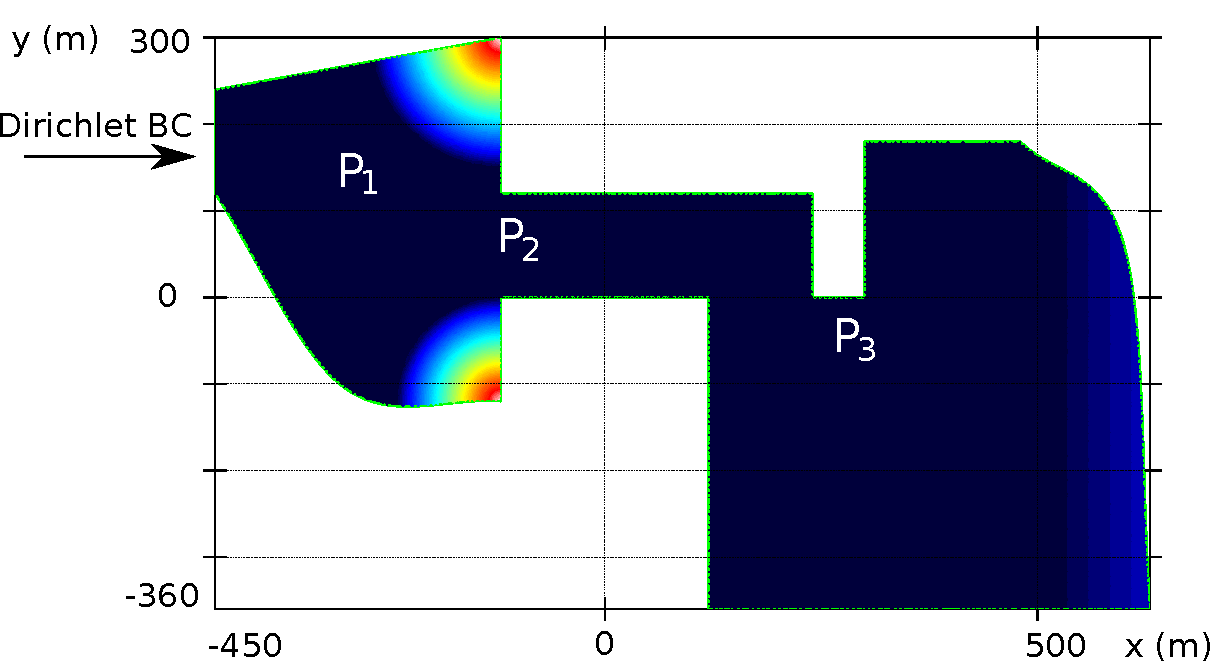
\includegraphics[width=\largefig]{chapters/lopes/pdf/sponge.pdf}
\caption{Sponge layer (viscosity $\nu(x,y) [{\tt Max} \approx 0.1\,{\tt m}^2{\tt
s}^{-1}, {\tt min}=0 \,{\tt m}^2{\tt s}^{-1}]$.}\label{lopes:fig:sponge}\par}
\end{figure}
\begin{figure}[!htb]
{\centering
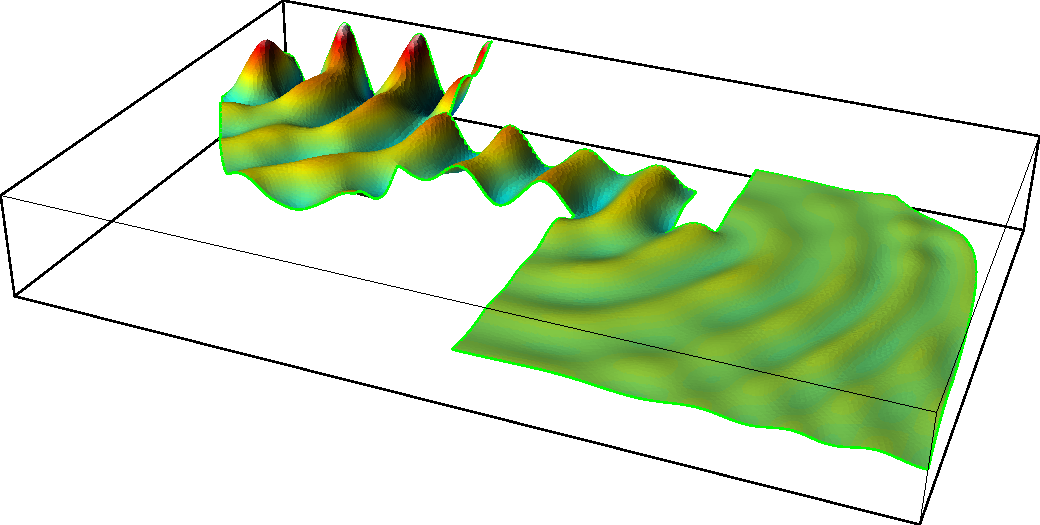
\includegraphics[width=\largefig]{chapters/lopes/pdf/eta.pdf}
\caption{Surface elevation $[{\tt Max}\approx 0.63\,{\tt
m}, {\tt min}\approx-0.73\,{\tt m}]$.}\label{lopes:fig:elevation}\par}
\end{figure}
\begin{figure}[!htb]
{\centering
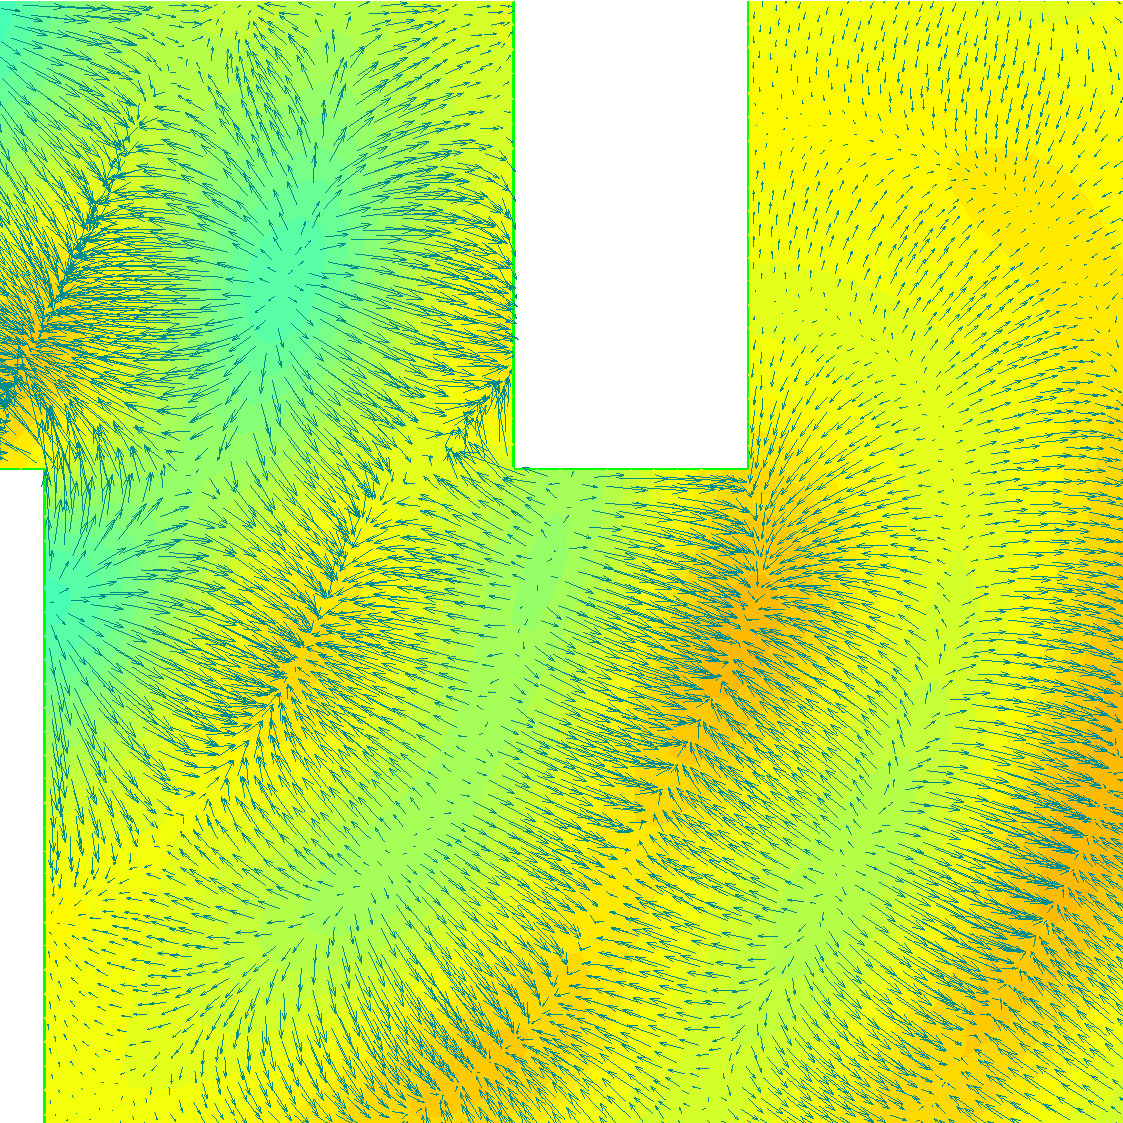
\includegraphics[width=\largefig]{chapters/lopes/pdf/pvel2.pdf}
\caption{Velocity vector field at $z=0$ and potential
$\phi_0(x,y,t_s)$ near $P_3$.
Potential values in $\Omega : [{\tt Max}\approx 14.2\,{\tt m}^{2}{\tt s}^{-1}, {\tt min}=-12.8\, {\tt m}^{2}{\tt s}^{-1}]$.}
\label{lopes:fig:potential1}\par}
\end{figure}
\begin{figure}[!htb]
{\centering
%\psfrag{m}[lb][rb]{$\eta$ $({\tt m})$}
%\psfrag{time}[lt][lt]{$t$ $({\tt s})$}
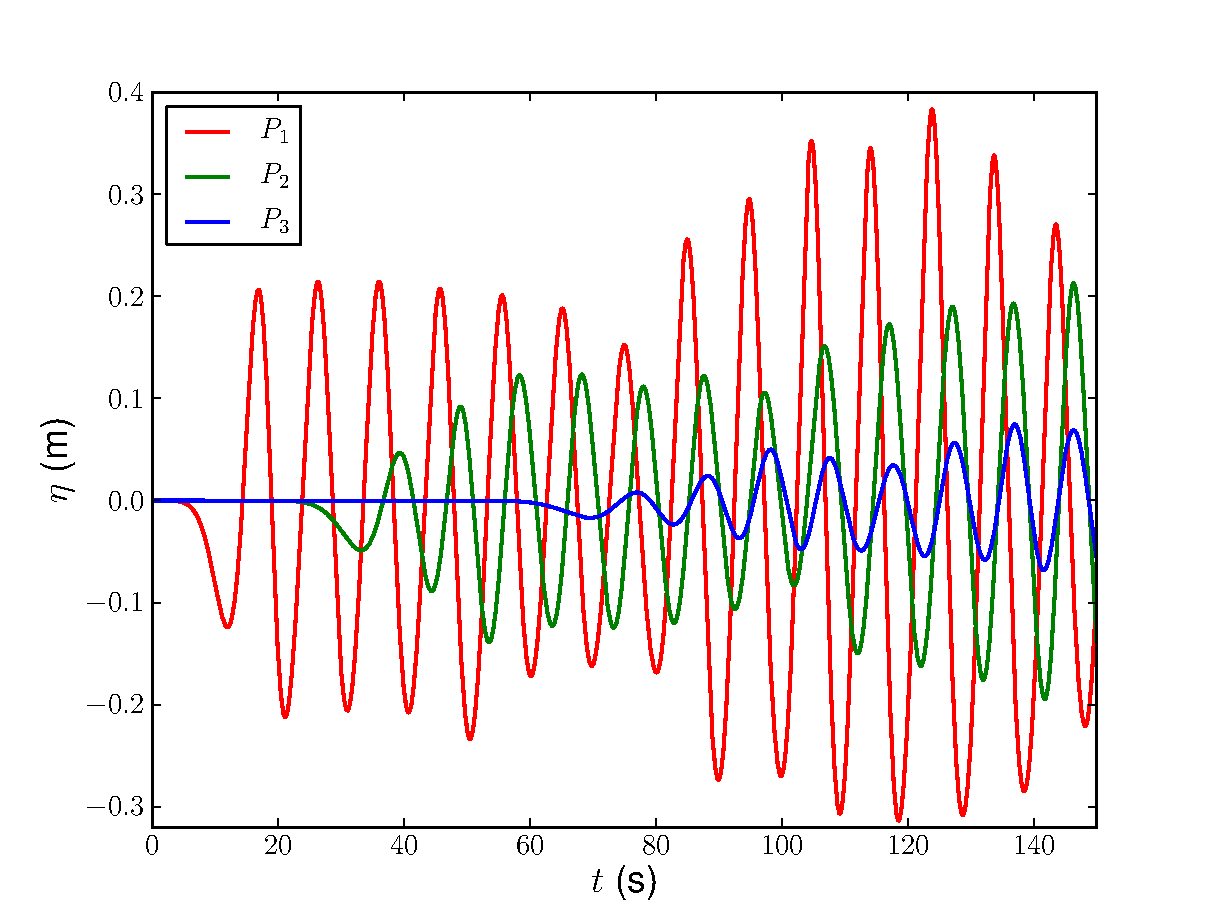
\includegraphics[width=\largefig]{chapters/lopes/pdf/etaprofile.pdf}
\caption{Surface elevation at $P_1$, $P_2$ and $P_3$ $[{\tt Max}\approx 0.4\, {\tt m}, {\tt min}=-0.31\,{\tt m}]$.}\label{lopes:fig:etap}\par}
\end{figure}
\begin{figure}[!htb]
{\centering
%\psfrag{m/s}[lb][rb]{$|\nabla \phi_0|$ $({\tt m\,s}^{-1})$}
%\psfrag{time}[lt][lt]{$t$ $({\tt s})$}
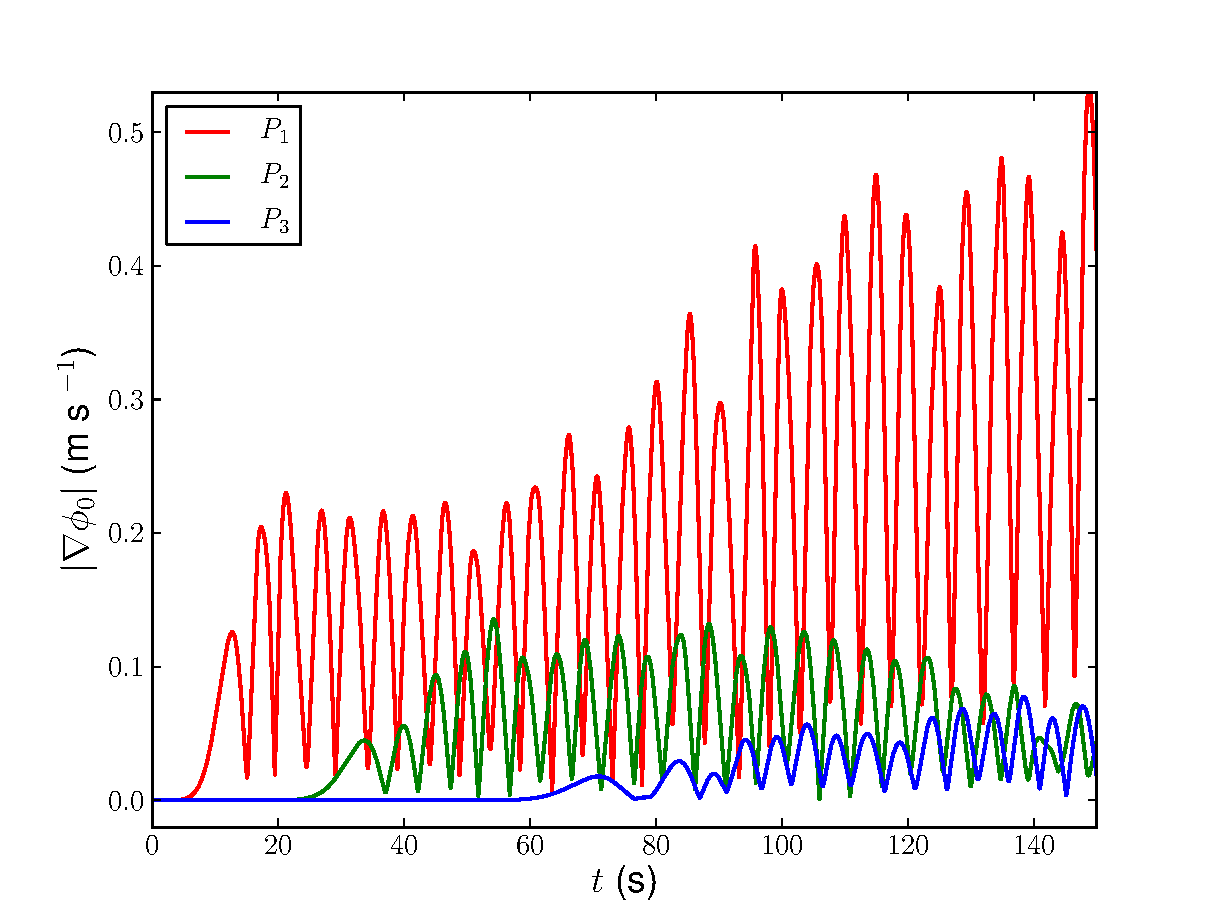
\includegraphics[width=\largefig]{chapters/lopes/pdf/velprofile.pdf}
\caption{Water speed  at $P_1$, $P_2$ and $P_3$
$[{\tt Max}\approx 0.53\, {\tt m\, s}^{-1}, {\tt min}=0\,{\tt m\, s}^{-1}]$.}\label{lopes:fig:velp}\par}
\end{figure}

From these numerical results, one can conclude that the
interaction between incident and reflected waves, near the harbour entrance,
 can generate wave amplitudes that  almost  take the
 triple value  of the incident wave amplitude.
One can also observe an analogous behaviour for
velocities.
Note that no
mechanism for releasing energy of the reflected waves
throughout the incident wave boundary is considered.
%}}}

%{{{ Conclusions and future work

\section{Conclusions and future work}

As far as we know,  the finite element
method is not often applied in surface water wave models
based on the BEP formulation.
In general, finite difference methods are preferred, since
they could be easily applied to higher-order equations.
On the  other hand, they are not appropriated for the
treatment of complex geometries, like those of harbours,
for instance.

In fact, the surface water wave problems are associated with
Boussinesq-type governing equations, which require very high order
\((\geq 6)\) spatial
derivatives or a very high number of equations \((\geq 6)\).
A first approach, to the high-order  models  using
discontinuous Galerkin finite element methods, can be found
in \cite{Engsig-KarupHesthavenEtAl2006}.

From this work one can conclude that the \fenics\, packages,
namely \dolfin\, and \ffc, are appropriated to model surface
water waves.

We have been developing \dolfwave, i.e., a \fenics\,
based application for BEP models (see {\tt http://www.fenics.org/wiki/DOLFWAVE}).
\dolfwave\, will also be compatible with  Xd3d
post-processor\footnote{{\tt
http://www.cmap.polytechnique.fr/\(\sim\)jouve/xd3d/}}.

The current state of the work, along with several numerical simulations, can be found  at  {\tt http://ptmat.fc.ul.pt/\(\sim\)ndl}.
This package will include some  standard potential models of low
 order  \((\leq 4)\)   as well as other new models to be submitted
elsewhere by the authors \cite{N.LopesP.PereiraEtAl}.
%}}}

%{{{Ackowledgments

\section{Acknowledgments}
L. Trabucho work is partially supported by Funda\c{c}\~{a}o para
a Ci\^{e}ncia e Tecnologia,
Financiamento Base 2008-ISFL-1-209.
N. Lopes work is supported by  Instituto Superior de
Engenharia de Lisboa -- ISEL.

\begin{center}
N. Lopes\(^{\ast,\diamond,\dagger}\), {\tt e-mail}: ndl@ptmat.fc.ul.pt\\
\quad P. Pereira\(^{\ast,\sharp}\),{\tt e-mail}: ppereira@deq.isel.ipl.pt\\
L. Trabucho\(^{\diamond,\dagger}\),{\tt e-mail}: trabucho@ptmat.fc.ul.pt
\end{center}
\vskip0.2in
{
\noindent \(^{\ast}\) \'{A}rea Cient\'{i}fica de Matem\'{a}tica\\
ISEL-Instituto Superior de Engenharia de Lisboa,
\\
Rua Conselheiro Em\'{i}dio Navarro, 1\\
1959-007 Lisboa\\
Portugal\\
}
\vskip0.2in
{
\noindent \(^{\diamond}\)
Departamento de Matem\'{a}tica\\
FCT-UNL-Faculdade de Ci\^{e}ncias e Tecnologia\\
2829-516 Caparica\\
Portugal\\
}
\vskip0.2in
{
\noindent \(^{\dagger}\)
CMAF-Centro de Matem\'{a}tica e Aplica\c{c}\~{o}es
Fundamentais,\\
Av. Prof. Gama Pinto, 2\\
1649-003 Lisboa,\\
Portugal
}
\vskip0.2in
{
\noindent \(^{\sharp}\)
CEFITEC-Centro de F\'{i}sica e Investiga\c{c}\~ao Tecnol\'{o}gica\\
FCT-UNL-Faculdade de Ci\^{e}ncias e Tecnologia\\
2829-516 Caparica\\
Portugal\\
}
\vfill

%}}}
\clearemptydoublepage}
\newcommand{\includeappendix}[1]{\include{appendix/#1}\clearemptydoublepage}
\newcommand{\includemisc}[1]{\include{#1}\clearemptydoublepage}

% Widths, use for figures
\newcommand{\largewidth}{10cm}
\newcommand{\smallwidth}{5cm}

% Project names
\newcommand{\projectfont}[1]{{#1}}
\newcommand{\ufl}{\projectfont{UFL}}
\newcommand{\sfc}{\projectfont{SFC}}
\newcommand{\ufc}{\projectfont{UFC}}
\newcommand{\ffc}{\projectfont{FFC}}
\newcommand{\pydolfin}{\projectfont{PyDOLFIN}}
\renewcommand{\dolfin}{\projectfont{DOLFIN}}
\renewcommand{\fenics}{\projectfont{FEniCS}}

% Package names
\newcommand{\packagefont}[1]{{#1}}
\newcommand{\numpy}{\packagefont{NumPy}}
\newcommand{\python}{\packagefont{python}}
\newcommand{\petsc}{\packagefont{PETSc}}
\newcommand{\diffsim}{\packagefont{diffsim}}
\newcommand{\tetgen}{\packagefont{TetGen}}
\newcommand{\emp}[1]{\texttt{#1}}
\newcommand{\bit}{\begin{itemize}}
\newcommand{\eit}{\end{itemize}}


% Notation macros
\newcommand{\dx}{\, \mathrm{d}x}
\newcommand{\dX}{\, \mathrm{d}X}
\newcommand{\ds}{\, \mathrm{d}s}
\newcommand{\dS}{\, \mathrm{d}S}
\newcommand{\dt}{\, \mathrm{d}t}
\newcommand{\R}{\mathbb{R}}
\newcommand{\Hdiv}{H(\mathrm{div})}
\newcommand{\Hcurl}{H(\mathrm{curl})}
\newcommand{\nedelec}{N\'ed\'elec}
\newcommand{\babuska}{Babu\v ska}

% Math operators
\DeclareMathOperator{\PEl}{PE_l}

% Example environment
\newtheorem{example}{Example}[chapter]

% Definition environment
\newtheorem{definition}{Definition}[chapter]

% Propopsition environment
\newtheorem{proposition}{Proposition}[section]

% Remark environment
\newtheorem{remark}{Remark}[section]

% Code environment
\DefineVerbatimEnvironment{code}{Verbatim}{frame=single,rulecolor=\color{blue}}

% Create index
\makeindex

% Start with empty pagestyle
\pagestyle{empty}
